\documentclass[svgnames]{llncs}

%\def\verbose{1}

\usepackage[paperwidth=15cm, paperheight=22cm, textwidth=12.2cm, textheight=19.3cm, inner=1.4cm, outer=1.4cm]{geometry}

\usepackage{JohnMath}
\usepackage{MathUnicode}

\usepackage{graphviz}
\usepackage{subfig}


\renewcommand{\rmdefault}{ptm}

\usepackage{framed}



%\theoremstyle{definition}
%\newtheorem{example}{Example}
%\newtheorem{remark}{Remark}
%\newtheorem{defn}{Definition}
% ...
%\theoremstyle{plain}
% ...

\usepackage{tikz}
\usetikzlibrary{arrows}
\usetikzlibrary{decorations.markings}
\usetikzlibrary{positioning}
\usetikzlibrary{shapes}
\usetikzlibrary{fit}
\usetikzlibrary{calc}
\usetikzlibrary{matrix}
\usetikzlibrary{backgrounds}

%\pgfdeclarelayer{background}
\pgfdeclarelayer{foreground}
\pgfsetlayers{background,main,foreground}

% BEGIN TIKZ GRID CODE
\makeatletter
\newif\if@showgrid@grid
\newif\if@showgrid@left
\newif\if@showgrid@right
\newif\if@showgrid@below
\newif\if@showgrid@above
\tikzset{%
    every show grid/.style={},
    show grid/.style={execute at end picture={\@showgrid{grid=true,#1}}},%
    show grid/.default={true},
    show grid/.cd,
    labels/.style={font={\sffamily\small},help lines,text=red!40},
    xlabels/.style={},
    ylabels/.style={},
    keep bb/.code={\useasboundingbox (current bounding box.south west) rectangle (current bounding box.north west);},
    true/.style={left,below},
    false/.style={left=false,right=false,above=false,below=false,grid=false},
    none/.style={left=false,right=false,above=false,below=false},
    all/.style={left=true,right=true,above=true,below=true},
    grid/.is if=@showgrid@grid,
    left/.is if=@showgrid@left,
    right/.is if=@showgrid@right,
    below/.is if=@showgrid@below,
    above/.is if=@showgrid@above,
    false,
}

\def\@showgrid#1{%
    \begin{scope}[every show grid,show grid/.cd,#1]
    \if@showgrid@grid
    \begin{pgfonlayer}{background}
    \draw [help lines, draw=red!10, step=1mm]
        (current bounding box.south west) grid
        (current bounding box.north east);
    \draw [help lines, draw=red!20, step=10mm]
        (current bounding box.south west) grid
        (current bounding box.north east);
%
    \pgfpointxy{1}{1}%
    \edef\xs{\the\pgf@x}%
    \edef\ys{\the\pgf@y}%
    \pgfpointanchor{current bounding box}{south west}
    \edef\xa{\the\pgf@x}%
    \edef\ya{\the\pgf@y}%
    \pgfpointanchor{current bounding box}{north east}
    \edef\xb{\the\pgf@x}%
    \edef\yb{\the\pgf@y}%
    \pgfmathtruncatemacro\xbeg{ceil(\xa/\xs)}
    \pgfmathtruncatemacro\xend{floor(\xb/\xs)}
    \if@showgrid@below
    \foreach \X in {\xbeg,...,\xend} {
      \pgfmathparse{int(mod(\X,10))}
      \ifnum\pgfmathresult=0
        \node [below,show grid/labels,show grid/xlabels] at (\X,\ya) {\X};
      \else\fi
    }
    \fi
    \if@showgrid@above
    \foreach \X in {\xbeg,...,\xend} {
      \pgfmathparse{int(mod(\X,10))}
      \ifnum\pgfmathresult=0
        \node [above,show grid/labels,show grid/xlabels] at (\X,\yb) {\X};
      \else\fi
    }
    \fi
    \pgfmathtruncatemacro\ybeg{ceil(\ya/\ys)}
    \pgfmathtruncatemacro\yend{floor(\yb/\ys)}
    \if@showgrid@left
    \foreach \Y in {\ybeg,...,\yend} {
      \pgfmathparse{int(mod(\Y,10))}
      \ifnum\pgfmathresult=0
        \node [left,show grid/labels,show grid/ylabels] at (\xa,\Y) {\Y};
      \else\fi
    }
    \fi
    \if@showgrid@right
    \foreach \Y in {\ybeg,...,\yend} {
      \pgfmathparse{int(mod(\Y,10))}
      \ifnum\pgfmathresult=0
        \node [right,show grid/labels,show grid/ylabels] at (\xb,\Y) {\Y};
      \else\fi
    }
    \fi
    \end{pgfonlayer}
    \fi
    \end{scope}
}
\makeatother
% END TIKZ GRID CODE


\begin{document}

\title{Ribbon proofs and dynamically scoped quantifiers}

\author{John Wickerson}
\institute{Technische Universität Berlin, Germany}

% make the title area
\maketitle

\newcommand{\ml}[2][t]{\mbox{\mdseries\begin{tabular}[#1]{@{}L@{}}#2\end{tabular}}}
\renewcommand{\ran}{\mathop{\rm ran}}



\section{Introduction}

A graphical proof system, called \emph{ribbon proofs}, for the propositional fragment of the logic of bunched implications was introduced by Bean~\cite{bean06}. Recently, Wickerson et al.\ upgraded ribbon proofs to a program logic by adding support for commands and existential quantifiers~\cite{wickerson+13}. An existential quantifier is handled in a ribbon proof by drawing an `existential box', labelled with the name of the variable being quantified, around a portion of the diagram. In their formalisation of ribbon proofs, Wickerson et al.\ assume that existential boxes are rectangular and well-nested. In practice, however, these boxes often partially overlap, or form more curious polygons than rectangles. Wickerson et al.\ mitigate this discrepancy between theory and practice by pointing out that overlapping polygons can be transformed into nested rectangles. Nevertheless, it is somewhat dissatisfying not to have a semantics for ribbon proofs directly. 

This paper describes a direct semantics for ribbon proofs whose existential boxes may be non-rectangular and may overlap. In doing so, we hope to provide a deeper understanding of this `intriguing proof structure'~\cite{wickerson+13}.

\subsubsection*{Outline} Section~\ref{sect:starting_point} explains the problem with the current semantics for ribbon proofs. Section~\ref{sect:main_ideas} explains the new semantics, which involves dynamically-scoped quantifiers. Section~\ref{sect:discussion} debates the importance of this new semantics, and the need for existential boxes at all. Section~\ref{sect:dynamically_scoped_quantifiers} describes the idea of dynamically-scoped quantifiers in the more general setting of first-order logic. Section~\ref{sect:semantics} proposes a semantics for dynamically-scoped quantifiers. Section~\ref{sect:related} contains pointers to related work. 

\section{Starting point}\label{sect:starting_point}

\def\comheight{5}
\def\comtextheight{\comheight/2}
\def\comtextleft{2}
\def\ribtextheight{3}

\newcommand{\mkRibbon}[5]{\fill[black!10] (#1,#2) rectangle (#3,#4);
\node at (#1/2+#3/2,#2+\ribtextheight) {#5}}
\newcommand{\mkStep}[4]{\fill[black!50] (#1,#2) rectangle (#3,#2+\comheight);
\node[anchor=west,text=white] at (#1+\comtextleft,#2+\comtextheight) {#4}}


Figure~\ref{fig:ribbonproof1} shows a little ribbon proof.

The proof depicts a pattern that commonly arises when verifying a while-loop. Prior to the loop, we establish the loop invariant $∃α.∃β.I$. Upon entering the loop body, we assume the test condition $b$. We then bring $b$ into the scope of the $α$ and $β$ quantifiers; this operation is sensible since $b$ (which is part of the program text) cannot mention the logical variables $α$ or $β$ (which exist only in the proof). We perform the loop body command $C_1$, which, in this case, produces three postconditions, $p_1$ and $p_2$ and $p_3$. We commute the scopes of the logical variables, to bring $α$ inside the scope of $β$, and then pick a new witness for $α$. The `Pick new $α$' step consumes $α$'s existential box, and produces a new one below. We then commute the logical variable scopes again, to bring $α$ back outside the scope of $β$, and pick a new witness for $β$. In doing so, we reestablish the loop invariant. After the loop, we assume the negation of the test condition, $¬b$.

\begin{figure}
\begin{center}
\input{dynquants_fig_ribbonproof1}
\end{center}
\caption{A ribbon proof}
\label{fig:ribbonproof1}
\end{figure}

\clearpage

Let us now examine the semantics of such a picture. The formal language of ribbon proofs given in previous work~\cite{wickerson+13} does not permit existential boxes to assume the exotic shapes seen in Fig.~\ref{fig:ribbonproof1}. The `scope extension' steps and the `commuting' steps are not allowed. They must be `desugared' according to the following transformations:

\begin{center}
\def\myblue{blue}
\def\myred{red}
\small $\begin{array}{rclrcl}
\begin{array}{@{}l@{}}
\begin{tikzpicture}[x=1mm,y=1mm,scale=1.]
\draw [rounded corners = 0.8mm, line width =0.15mm, \myblue] (12.15,0.) -- (12.15,0.);
\draw [rounded corners = 0.8mm, line width =0.15mm, \myblue] (20.85,0.) -- (20.85,0.);
\draw [rounded corners = 0.8mm, line width =0.15mm, \myblue] (12.15,-7.) -- (12.15,0.);
\draw [rounded corners = 0.8mm, line width =0.15mm, \myblue] (20.85,-7.) -- (20.85,0.);
\draw [line width = 0.5mm, white] (3.,0.) -- (3.,-7.);
\draw [line width = 0.5mm, white] (8.,0.) -- (8.,-7.);
\fill [black!15] (3.,0.) -- (3.,-7.) -- (8.,-7.) -- (8.,0.) -- cycle;
\draw [black] (5.5,-3.) node{\smash{$\ml[t]{p}$}};
\draw [line width = 0.5mm, white] (14.,0.) -- (14.,-7.);
\draw [line width = 0.5mm, white] (19.,0.) -- (19.,-7.);
\fill [black!15] (14.,0.) -- (14.,-7.) -- (19.,-7.) -- (19.,0.) -- cycle;
\draw [black] (16.5,-3.) node{\smash{$\ml[t]{q}$}};
\draw [line width = 0.5mm, white] (14.,-7.) -- (14.,-7.);
\draw [line width = 0.5mm, white] (19.,-7.) -- (19.,-7.);
\fill [black!15] (14.,-7.) -- (14.,-7.) -- (19.,-7.) -- (19.,-7.) -- cycle;
\draw [line width = 0.5mm, white] (3.,-7.) -- (3.,-7.);
\draw [line width = 0.5mm, white] (8.,-7.) -- (8.,-7.);
\fill [black!15] (3.,-7.) -- (3.,-7.) -- (8.,-7.) -- (8.,-7.) -- cycle;
\draw [rounded corners = 0.8mm, line width =0.15mm, \myblue] (12.15,-7.) -- (12.15,-7.);
\draw [rounded corners = 0.8mm, line width =0.15mm, \myblue] (20.85,-7.) -- (20.85,-7.);
\draw [line width = 0.5mm, white] (14.,-7.) -- (14.,-9.);
\draw [line width = 0.5mm, white] (19.,-7.) -- (19.,-9.);
\fill [black!15] (14.,-7.) -- (14.,-9.) -- (19.,-9.) -- (19.,-7.) -- cycle;
\draw [line width = 0.5mm, white] (3.,-7.) -- (3.,-9.);
\draw [line width = 0.5mm, white] (8.,-7.) -- (8.,-9.);
\fill [black!15] (3.,-7.) -- (3.,-9.) -- (8.,-9.) -- (8.,-7.) -- cycle;
\draw [rounded corners = 0.8mm, line width =0.15mm, \myblue] (1.15,-9.) -- (1.15,-8.) -- (12.15,-8.) -- (12.15,-7.);
\draw [rounded corners = 0.8mm, line width =0.15mm, \myblue] (20.85,-9.) -- (20.85,-7.);
\draw [line width = 0.5mm, white] (14.,-9.) -- (14.,-17.);
\draw [line width = 0.5mm, white] (19.,-9.) -- (19.,-17.);
\fill [black!15] (14.,-9.) -- (14.,-17.) -- (19.,-17.) -- (19.,-9.) -- cycle;
\draw [line width = 0.5mm, white] (3.,-9.) -- (3.,-17.);
\draw [line width = 0.5mm, white] (8.,-9.) -- (8.,-17.);
\fill [black!15] (3.,-9.) -- (3.,-17.) -- (8.,-17.) -- (8.,-9.) -- cycle;
\draw [rounded corners = 0.8mm, line width =0.15mm, \myblue] (1.15,-17.) -- (1.15,-9.);
\draw [rounded corners = 0.8mm, line width =0.15mm, \myblue] (20.85,-17.) -- (20.85,-9.);
\fill [white] (11.,-1.3) -- (11.,-4.8) -- (14.,-4.8) -- (14.,-1.3) -- cycle;
\draw [black] (8.,-3.) node[anchor=west]{$∃x$};
\end{tikzpicture}
\end{array}
&~≝&\!\!\! 
\begin{array}{@{}l@{}}
\begin{tikzpicture}[x=1mm,y=1mm,scale=1.]
\draw [rounded corners = 0.8mm, line width =0.15mm, \myblue] (15.15,0.) -- (15.15,0.);
\draw [rounded corners = 0.8mm, line width =0.15mm, \myblue] (23.85,0.) -- (23.85,0.);
\draw [rounded corners = 0.8mm, line width =0.15mm, \myblue] (15.15,-5.) -- (15.15,0.);
\draw [rounded corners = 0.8mm, line width =0.15mm, \myblue] (23.85,-5.) -- (23.85,0.);
\draw [line width = 0.5mm, white] (3.,0.) -- (3.,-5.);
\draw [line width = 0.5mm, white] (8.,0.) -- (8.,-5.);
\fill [black!15] (3.,0.) -- (3.,-5.) -- (8.,-5.) -- (8.,0.) -- cycle;
\draw [black] (5.5,-3.) node{\smash{$\ml[t]{p}$}};
\draw [line width = 0.5mm, white] (17.,0.) -- (17.,-5.);
\draw [line width = 0.5mm, white] (22.,0.) -- (22.,-5.);
\fill [black!15] (17.,0.) -- (17.,-5.) -- (22.,-5.) -- (22.,0.) -- cycle;
\draw [black] (19.5,-3.) node{\smash{$\ml[t]{q}$}};
\draw [line width = 0.5mm, white] (17.,-5.) -- (17.,-5.);
\draw [line width = 0.5mm, white] (22.,-5.) -- (22.,-5.);
\fill [black!15] (17.,-5.) -- (17.,-5.) -- (22.,-5.) -- (22.,-5.) -- cycle;
\draw [line width = 0.5mm, white] (3.,-5.) -- (3.,-5.);
\draw [line width = 0.5mm, white] (8.,-5.) -- (8.,-5.);
\fill [black!15] (3.,-5.) -- (3.,-5.) -- (8.,-5.) -- (8.,-5.) -- cycle;
\draw [rounded corners = 0.8mm, line width =0.15mm, \myblue] (15.15,-5.) -- (15.15,-5.);
\draw [rounded corners = 0.8mm, line width =0.15mm, \myblue] (23.85,-5.) -- (23.85,-5.);
\draw [rounded corners = 0.8mm, line width =0.15mm, \myblue] (15.15,-6.) -- (15.15,-5.);
\draw [rounded corners = 0.8mm, line width =0.15mm, \myblue] (23.85,-6.) -- (23.85,-5.);
\draw [line width = 0.5mm, white] (17.,-5.) -- (17.,-6.);
\draw [line width = 0.5mm, white] (22.,-5.) -- (22.,-6.);
\fill [black!15] (17.,-5.) -- (17.,-6.) -- (22.,-6.) -- (22.,-5.) -- cycle;
\draw [line width = 0.5mm, white] (3.,-5.) -- (3.,-6.);
\draw [line width = 0.5mm, white] (8.,-5.) -- (8.,-6.);
\fill [black!15] (3.,-5.) -- (3.,-6.) -- (8.,-6.) -- (8.,-5.) -- cycle;
\fill[fill=black!55] (1.,-11.) rectangle (24.,-6.);
\draw [white] (1.,-8.5) node[anchor=west]{\begin{tabular}{@{\hspace{-0.8mm}}l@{\hspace{-0.8mm}}}Extend $x$'s scope\end{tabular}};
\draw [rounded corners = 0.8mm, line width =0.15mm, \myblue] (1.15,-11.) -- (1.15,-11.);
\draw [rounded corners = 0.8mm, line width =0.15mm, \myblue] (23.85,-11.) -- (23.85,-11.);
\draw [rounded corners = 0.8mm, line width =0.15mm, \myblue] (1.15,-11.) -- (1.15,-11.);
\draw [rounded corners = 0.8mm, line width =0.15mm, \myblue] (23.85,-11.) -- (23.85,-11.);
\draw [rounded corners = 0.8mm, line width =0.15mm, \myblue] (1.15,-17.) -- (1.15,-11.);
\draw [rounded corners = 0.8mm, line width =0.15mm, \myblue] (23.85,-17.) -- (23.85,-11.);
\draw [line width = 0.5mm, white] (3.,-11.) -- (3.,-17.);
\draw [line width = 0.5mm, white] (8.,-11.) -- (8.,-17.);
\fill [black!15] (3.,-11.) -- (3.,-17.) -- (8.,-17.) -- (8.,-11.) -- cycle;
\draw [black] (5.5,-14.) node{\smash{$\ml[t]{p}$}};
\draw [line width = 0.5mm, white] (17.,-11.) -- (17.,-17.);
\draw [line width = 0.5mm, white] (22.,-11.) -- (22.,-17.);
\fill [black!15] (17.,-11.) -- (17.,-17.) -- (22.,-17.) -- (22.,-11.) -- cycle;
\draw [black] (19.5,-14.) node{\smash{$\ml[t]{q}$}};
\fill [white] (0.,-12.3) -- (0.,-15.8) -- (3.,-15.8) -- (3.,-12.3) -- cycle;
\draw [black] (-3.,-14.) node[anchor=west]{$∃x$};
\fill [white] (14.,-1.3) -- (14.,-4.8) -- (17.,-4.8) -- (17.,-1.3) -- cycle;
\draw [black] (11.,-3.) node[anchor=west]{$∃x$};
\end{tikzpicture}
\end{array} \begin{array}{l}\text{if $x$ is} \\ \text{not free} \\ \text{in $p$}
\end{array}
~~~~ &~~~~
\begin{array}{@{}l@{}}
\begin{tikzpicture}[x=1mm,y=1mm,scale=1.]
\draw [rounded corners = 0.8mm, line width =0.15mm, \myblue] (3.15,0.) -- (3.15,0.);
\draw [rounded corners = 0.8mm, line width =0.15mm, \myblue] (18.85,0.) -- (18.85,0.);
\draw [rounded corners = 0.8mm, line width =0.15mm, \myred] (8.15,0.) -- (8.15,0.);
\draw [rounded corners = 0.8mm, line width =0.15mm, \myred] (16.85,0.) -- (16.85,0.);
\draw [rounded corners = 0.8mm, line width =0.15mm, \myblue] (3.15,-7.) -- (3.15,0.);
\draw [rounded corners = 0.8mm, line width =0.15mm, \myblue] (18.85,-7.) -- (18.85,0.);
\draw [rounded corners = 0.8mm, line width =0.15mm, \myred] (8.15,-7.) -- (8.15,0.);
\draw [rounded corners = 0.8mm, line width =0.15mm, \myred] (16.85,-7.) -- (16.85,0.);
\draw [line width = 0.5mm, white] (10.,0.) -- (10.,-7.);
\draw [line width = 0.5mm, white] (15.,0.) -- (15.,-7.);
\fill [black!15] (10.,0.) -- (10.,-7.) -- (15.,-7.) -- (15.,0.) -- cycle;
\draw [black] (12.5,-3.) node{\smash{$\ml[t]{p}$}};
\draw [line width = 0.5mm, white] (10.,-7.) -- (10.,-7.);
\draw [line width = 0.5mm, white] (15.,-7.) -- (15.,-7.);
\fill [black!15] (10.,-7.) -- (10.,-7.) -- (15.,-7.) -- (15.,-7.) -- cycle;
\draw [rounded corners = 0.8mm, line width =0.15mm, \myblue] (3.15,-7.) -- (3.15,-7.);
\draw [rounded corners = 0.8mm, line width =0.15mm, \myblue] (18.85,-7.) -- (18.85,-7.);
\draw [rounded corners = 0.8mm, line width =0.15mm, \myred] (8.15,-7.) -- (8.15,-7.);
\draw [rounded corners = 0.8mm, line width =0.15mm, \myred] (16.85,-7.) -- (16.85,-7.);
\draw [line width = 0.5mm, white] (10.,-7.) -- (10.,-9.);
\draw [line width = 0.5mm, white] (15.,-7.) -- (15.,-9.);
\fill [black!15] (10.,-7.) -- (10.,-9.) -- (15.,-9.) -- (15.,-7.) -- cycle;
\draw [rounded corners = 0.8mm, line width =0.15mm, \myblue] (3.15,-9.) -- (3.15,-7.);
\draw [rounded corners = 0.8mm, line width =0.15mm, \myblue] (18.85,-9.) -- (18.85,-7.);
\draw [rounded corners = 0.8mm, line width =0.15mm, \myred] (1.15,-9.) -- (1.15,-8.) -- (8.15,-8.) -- (8.15,-7.);
\draw [rounded corners = 0.8mm, line width =0.15mm, \myred] (20.85,-9.) -- (20.85,-8.) -- (16.85,-8.) -- (16.85,-7.);
\draw [line width = 0.5mm, white] (10.,-9.) -- (10.,-16.);
\draw [line width = 0.5mm, white] (15.,-9.) -- (15.,-16.);
\fill [black!15] (10.,-9.) -- (10.,-16.) -- (15.,-16.) -- (15.,-9.) -- cycle;
\draw [rounded corners = 0.8mm, line width =0.15mm, \myred] (1.15,-16.) -- (1.15,-9.);
\draw [rounded corners = 0.8mm, line width =0.15mm, \myred] (20.85,-16.) -- (20.85,-9.);
\draw [rounded corners = 0.8mm, line width =0.15mm, \myblue] (3.15,-16.) -- (3.15,-9.);
\draw [rounded corners = 0.8mm, line width =0.15mm, \myblue] (18.85,-16.) -- (18.85,-9.);
\fill [white] (7.,-1.3) -- (7.,-4.8) -- (10.,-4.8) -- (10.,-1.3) -- cycle;
\draw [black] (4.,-3.) node[anchor=west]{$∃y$};
\fill [white] (2.,-1.3) -- (2.,-4.8) -- (5.,-4.8) -- (5.,-1.3) -- cycle;
\draw [black] (-1.,-3.) node[anchor=west]{$∃x$};
\end{tikzpicture}
\end{array} 
&~≝&\!\!\!
\begin{array}{@{}l@{}}
\begin{tikzpicture}[x=1mm,y=1mm,scale=1.]
\draw [rounded corners = 0.8mm, line width =0.15mm, \myblue] (1.15,0.) -- (1.15,0.);
\draw [rounded corners = 0.8mm, line width =0.15mm, \myblue] (18.85,0.) -- (18.85,0.);
\draw [rounded corners = 0.8mm, line width =0.15mm, \myred] (8.15,0.) -- (8.15,0.);
\draw [rounded corners = 0.8mm, line width =0.15mm, \myred] (16.85,0.) -- (16.85,0.);
\draw [rounded corners = 0.8mm, line width =0.15mm, \myblue] (1.15,-5.) -- (1.15,0.);
\draw [rounded corners = 0.8mm, line width =0.15mm, \myblue] (18.85,-5.) -- (18.85,0.);
\draw [rounded corners = 0.8mm, line width =0.15mm, \myred] (8.15,-5.) -- (8.15,0.);
\draw [rounded corners = 0.8mm, line width =0.15mm, \myred] (16.85,-5.) -- (16.85,0.);
\draw [line width = 0.5mm, white] (10.,0.) -- (10.,-5.);
\draw [line width = 0.5mm, white] (15.,0.) -- (15.,-5.);
\fill [black!15] (10.,0.) -- (10.,-5.) -- (15.,-5.) -- (15.,0.) -- cycle;
\draw [black] (12.5,-3.) node{\smash{$\ml[t]{p}$}};
\draw [line width = 0.5mm, white] (10.,-5.) -- (10.,-5.);
\draw [line width = 0.5mm, white] (15.,-5.) -- (15.,-5.);
\fill [black!15] (10.,-5.) -- (10.,-5.) -- (15.,-5.) -- (15.,-5.) -- cycle;
\draw [rounded corners = 0.8mm, line width =0.15mm, \myblue] (1.15,-5.) -- (1.15,-5.);
\draw [rounded corners = 0.8mm, line width =0.15mm, \myblue] (18.85,-5.) -- (18.85,-5.);
\draw [rounded corners = 0.8mm, line width =0.15mm, \myred] (8.15,-5.) -- (8.15,-5.);
\draw [rounded corners = 0.8mm, line width =0.15mm, \myred] (16.85,-5.) -- (16.85,-5.);
\draw [rounded corners = 0.8mm, line width =0.15mm, \myblue] (1.15,-6.) -- (1.15,-5.);
\draw [rounded corners = 0.8mm, line width =0.15mm, \myblue] (18.85,-6.) -- (18.85,-5.);
\draw [rounded corners = 0.8mm, line width =0.15mm, \myred] (8.15,-6.) -- (8.15,-5.);
\draw [rounded corners = 0.8mm, line width =0.15mm, \myred] (16.85,-6.) -- (16.85,-5.);
\draw [line width = 0.5mm, white] (10.,-5.) -- (10.,-6.);
\draw [line width = 0.5mm, white] (15.,-5.) -- (15.,-6.);
\fill [black!15] (10.,-5.) -- (10.,-6.) -- (15.,-6.) -- (15.,-5.) -- cycle;
\fill[fill=black!55] (1.,-10.) rectangle (19.,-6.);
\draw [white] (1.,-8.) node[anchor=west]{\begin{tabular}{@{\hspace{-0.8mm}}l@{\hspace{-0.8mm}}}Swap $x$ and $y$\end{tabular}};
\draw [rounded corners = 0.8mm, line width =0.15mm, \myblue] (8.15,-10.) -- (8.15,-10.);
\draw [rounded corners = 0.8mm, line width =0.15mm, \myblue] (16.85,-10.) -- (16.85,-10.);
\draw [rounded corners = 0.8mm, line width =0.15mm, \myred] (1.15,-10.) -- (1.15,-10.);
\draw [rounded corners = 0.8mm, line width =0.15mm, \myred] (18.85,-10.) -- (18.85,-10.);
\draw [rounded corners = 0.8mm, line width =0.15mm, \myblue] (8.15,-10.) -- (8.15,-10.);
\draw [rounded corners = 0.8mm, line width =0.15mm, \myblue] (16.85,-10.) -- (16.85,-10.);
\draw [rounded corners = 0.8mm, line width =0.15mm, \myred] (1.15,-10.) -- (1.15,-10.);
\draw [rounded corners = 0.8mm, line width =0.15mm, \myred] (18.85,-10.) -- (18.85,-10.);
\draw [rounded corners = 0.8mm, line width =0.15mm, \myblue] (8.15,-10.) -- (8.15,-10.);
\draw [rounded corners = 0.8mm, line width =0.15mm, \myblue] (16.85,-10.) -- (16.85,-10.);
\draw [rounded corners = 0.8mm, line width =0.15mm, \myred] (1.15,-10.) -- (1.15,-10.);
\draw [rounded corners = 0.8mm, line width =0.15mm, \myred] (18.85,-10.) -- (18.85,-10.);
\draw [rounded corners = 0.8mm, line width =0.15mm, \myblue] (8.15,-16.) -- (8.15,-10.);
\draw [rounded corners = 0.8mm, line width =0.15mm, \myblue] (16.85,-16.) -- (16.85,-10.);
\draw [rounded corners = 0.8mm, line width =0.15mm, \myred] (1.15,-16.) -- (1.15,-10.);
\draw [rounded corners = 0.8mm, line width =0.15mm, \myred] (18.85,-16.) -- (18.85,-10.);
\draw [line width = 0.5mm, white] (10.,-10.) -- (10.,-16.);
\draw [line width = 0.5mm, white] (15.,-10.) -- (15.,-16.);
\fill [black!15] (10.,-10.) -- (10.,-16.) -- (15.,-16.) -- (15.,-10.) -- cycle;
\draw [black] (12.5,-13.) node{\smash{$\ml[t]{p}$}};
\fill [white] (7.,-11.3) -- (7.,-14.8) -- (10.,-14.8) -- (10.,-11.3) -- cycle;
\draw [black] (4.,-13.) node[anchor=west]{$∃x$};
\fill [white] (0.,-11.3) -- (0.,-14.8) -- (3.,-14.8) -- (3.,-11.3) -- cycle;
\draw [black] (-3.,-13.) node[anchor=west]{$∃y$};
\fill [white] (7.,-1.3) -- (7.,-4.8) -- (10.,-4.8) -- (10.,-1.3) -- cycle;
\draw [black] (4.,-3.) node[anchor=west]{$∃y$};
\fill [white] (0.,-1.3) -- (0.,-4.8) -- (3.,-4.8) -- (3.,-1.3) -- cycle;
\draw [black] (-3.,-3.) node[anchor=west]{$∃x$};
\end{tikzpicture}
\end{array}
\end{array}$
\end{center}

\noindent We thus obtain the picture shown in Fig.~\ref{fig:ribbonproof2}. 

It is a shame that the picture has become significantly more complex, and that the interesting structure of overlapping quantifiers can no longer be easily seen.

Figure~\ref{fig:ribbonproof3} depicts how Fig.~\ref{fig:ribbonproof2} is then analysed as a graph. The graph has a hierarchical structure, in that loops and existential boxes are nodes that contain within them a complete graph. Besides this nesting hierarchy, we have a dag structure formed by the $⇒$-arrows. These arrows link commands to their pre- and postconditions.

\newcommand{\mkRibbonNode}[4]{\node[fill=black!10] (#1) at (#2,#3) {\vphantom{Ay}#4}}
\newcommand{\mkStepNode}[4]{\node[fill=black!50,text=white] (#1) at (#2,#3) {\vphantom{Ay}#4}}

\tikzset{preimplies/.style={-implies,double,double equal sign distance}}
\tikzset{postimplies/.style={double,double equal sign distance,-implies}}
\tikzset{quantifieredge/.style={->,>=stealth',dotted}}


\begin{figure}
\begin{center}
\begin{tabular}{ll}
\subfloat[A ribbon proof, with scope-extending and scope-commuting shown as explicit proof steps]{
\input{dynquants_fig_ribbonproof2}
\label{fig:ribbonproof2}
}
& 
\subfloat[The corresponding graph]{
\scalebox{0.77}{\input{dynquants_fig_ribbonproof33}}
\label{fig:ribbonproof33}
}
\end{tabular}
\end{center}
\caption{}
\label{fig:ribbonproof2and33}
\end{figure}

\clearpage

\section{Main ideas}\label{sect:main_ideas}

In this section, we shall describe how to obtain a graphical semantics for pictures such as Fig.~\ref{fig:ribbonproof1}, that results in much more concise graphs than that shown in Fig.~\ref{fig:ribbonproof33}.

We shall proceed by a process of iterative refinement. Our first step is to flatten the existential boxes.

\subsection{Flattening existential boxes}

\begin{figure}
\begin{center}
\scalebox{0.77}{\input{dynquants_fig_ribbonproof3}}
\end{center}
\caption{First refinement: flattening existential boxes}
\label{fig:ribbonproof3}
\end{figure}

Figure~\ref{fig:ribbonproof3} is obtained from Fig.~\ref{fig:ribbonproof33} by replacing the existential boxes with single nodes, each of which is linked to the contents of the corresponding box by dotted arrows. We can think of this process as `unpacking' or `flattening' the existential boxes. Where previously the contents of each existential box was a completely separate graph, we now have nodes inside and outside the box co-existing in the same graph. (For now, we shall leave the loop-block as a special node that contains a complete graph.) 

Note that the dotted arrows form a tree structure; that is, no node is a \emph{direct} descendent of more than one existential quantifier. Previously, this `tree' property was enforced by the fact that existential boxes must be well-nested.

We have only linked each existential node to the \emph{assertion nodes} in its scope, not the \emph{command nodes}. This is our first Main Idea.

\begin{quote}\noindent 
{\bf Main Idea 1.} It is not necessary for command nodes to be located within the scope of existential quantifiers.
\end{quote}

\noindent To clarify: observe that at the bottom of Fig.~\ref{fig:ribbonproof33}, $C_2$ and $p_6$ are both visually inside $β$'s existential box. It is important that $p_6$ is within $β$'s scope, in case $p_6$ mentions $β$. But $C_2$, being a piece of program text, cannot mention logical variables, because these appear only in the proof. Therefore, at the bottom of Fig.~\ref{fig:ribbonproof3}, we \emph{do not} have a dotted arrow from $∃β$ to $C_2$, but we \emph{do} have one from $∃β$ to $p_6$.

\clearpage

\subsection{Relaxing the tree property}

In Fig.~\ref{fig:ribbonproof3}, the dotted arrows form a tree structure: each assertion node and each existential node is the target of at most one dotted arrow, and these arrows do not form cycles. Let us relax this constraint, and instead arrange that each assertion node receives an arrow \emph{directly} from those quantifiers that bind its variables. As such, an assertion node may have more than one `parent' in this dotted-arrow hierarchy. 
For instance, Fig.~\ref{fig:ribbonproof3} begins with
\begin{center}
\begin{tikzpicture}[x=1mm,y=-1mm]
\node[shape=circle,draw=red,inner sep=0.2mm] (a) at (0,0) {$∃α$};
\node[shape=circle,draw=green,inner sep=0.2mm] (b) at (9,0) {$∃β$};
\mkRibbonNode{n}{18}{0}{$I$};
\path (a) edge [quantifieredge] (b);
\path (b) edge [quantifieredge] (n);
\end{tikzpicture}
\end{center}

\noindent while Fig.~\ref{fig:ribbonproof4}, which is obtained from Fig.~\ref{fig:ribbonproof3} by relaxing the tree constraint, begins with
\begin{center}
\begin{tikzpicture}[x=1mm,y=-1mm]
\node[shape=circle,draw=red,inner sep=0.2mm] (a) at (0,3) {$∃α$};
\node[shape=circle,draw=green,inner sep=0.2mm] (b) at (9,-3) {$∃β$};
\mkRibbonNode{n}{18}{0}{$I$};
\path (a) edge [quantifieredge] (n);
\path (b) edge [quantifieredge] (n);
\end{tikzpicture}
\end{center}

\noindent Observe that we have removed the ordering between $∃α$ and $∃β$: they now both link to $I$, but not to each other. We have thus obtained a representation that is agnostic about the order of quantifiers. As such, the two `Commute...' steps in Fig.~\ref{fig:ribbonproof3} are no longer needed in Fig.~\ref{fig:ribbonproof4}. The `Extend scope...' steps from Fig.~\ref{fig:ribbonproof3} also become redundant, because we no longer have the concept of a variable scoping over a formula: instead the quantifiers link directly to those parts of the formula where the variable is used. In essence, we have moved from `statically-scoped quantifiers' to `dynamically-scoped quantifiers'.

\begin{quote}\noindent 
{\bf Main Idea 2.} Dynamically-scoped quantifiers, where each variable is linked directly to its binder, are more appropriate than statically-scoped quantifiers here.
\end{quote}

\begin{figure}
\begin{center}
\input{dynquants_fig_ribbonproof4}
\end{center}
\caption{Second refinement: relaxing the `tree' property on dotted arrows}
\label{fig:ribbonproof4}
\end{figure}

\noindent Figure~\ref{fig:ribbonproof4} captures the intention of the picture in Fig.~\ref{fig:ribbonproof1} quite well. However, there remains a little too much repetition. This repetition appears at the boundaries of the loop block, so we shall turn our attention to loops now.

\clearpage

\subsection{Flattening loop nodes}

The loop invariant
\begin{center}
\begin{tikzpicture}[x=1mm,y=-1mm]
\node[shape=circle,draw=red,inner sep=0.2mm] (a) at (0,3) {$∃α$};
\node[shape=circle,draw=green,inner sep=0.2mm] (b) at (9,-3) {$∃β$};
\mkRibbonNode{n}{18}{0}{$I$};
\path (a) edge [quantifieredge] (n);
\path (b) edge [quantifieredge] (n);
\end{tikzpicture}
\end{center}
appears in four places in Fig.~\ref{fig:ribbonproof4}: above the loop, at the top of the loop body, at the bottom of the loop body, and below the loop. In Fig.~\ref{fig:ribbonproof1}, this loop invariant appears only twice: once above the loop, and once at the bottom of the loop body; the other positions can be inferred. This repetition in Fig.~\ref{fig:ribbonproof4} results from the requirement that each loop block contains a complete, separate graph.

We have previously `flattened' existential boxes; let us now perform this same trick on loop blocks. Figure~\ref{fig:ribbonproof5} is the same as Fig.~\ref{fig:ribbonproof4}, but the loop block has been replaced by a single node labelled `\texttt{loop \{...\}}' that is linked to each command in the loop body by a solid grey arrow. 

Note that it is not necessary to link the `\texttt{loop \{...\}}' node to the \emph{assertions} that appear inside the loop body, only the \emph{commands}. (This is something of a reversal of Main Idea~1.)  This means that we no longer need one copy of the loop invariant just before the loop and one at the top of the loop body -- the same nodes can now be reused in both cases.

\begin{quote}\noindent 
{\bf Main Idea 3.} It is not necessary for assertion nodes to be located within the scope of loops.
\end{quote}

\noindent Note also that the loop node does not have pre- or postconditions. That is, no $⇒$-arrows enter or leave it. In fact, the only arrows that are permitted to connect to loop nodes are the solid grey ones. The loop invariant can still be deduced by inspecting the graph, however. 

\begin{figure}
\begin{center}
\begin{tabular}{ll}
\subfloat[A ribbon proof (repeated from Fig.~\ref{fig:ribbonproof1})]{
\scalebox{0.77}{\input{dynquants_fig_ribbonproof1}}
\label{fig:ribbonproof1again}
}
& 
\subfloat[Final refinement: flattening loop nodes]{
\scalebox{0.9}{\input{dynquants_fig_ribbonproof5}}
\label{fig:ribbonproof5}
}
\end{tabular}
\end{center}
\caption{}
\label{fig:ribbonproof5and1}
\end{figure}

\clearpage
\section{Discussion}\label{sect:discussion}

The refined graphs presented in the previous section seem to shed light on the `dynamic scoping of existential boxes' seen in ribbon proofs~\cite{wickerson+13}, and as such, the primary objective of this paper has been achieved. We must question, however, the practical utility of the observations reported in this paper.

First, the refined graphs are much harder to formalise, and hence to prove sound. What makes graphs such as the one in Fig.~\ref{fig:ribbonproof33} easier to work with is the fact that each loop node and each existential box contains a complete graph that is isolated from the rest of the diagram. In contrast, our refined graphs assemble all the nodes together as siblings, and allow arrows to pass between them quite freely, subject to some fairly subtle semantic constraints. This difficulty is surpassable, but initial investigations, using the Isabelle proof assistant, suggest that a considerable effort is required.

Second, we must ask whether our refined graphs are needed at all, when there exists an alternative semantics for ribbon proofs that does not involve graphs at all. Wickerson et al.~\cite{wickerson+13} describe two formalisations of ribbon proofs: a `stratified' version, which is sensitive to the particular layout of proof steps, and a `graphical' version, that considers only the connectivity between the proof steps, ignoring their layout. The stratified semantics is the simpler of the two, does not require graphs, and does not require the `variables-as-resource' scheme. The advantage of the graphical semantics is that proofs can be identified up to graph isomorphism, and this can be helpful when, for instance, analysing dependencies within the proof. If ribbon proofs prove helpful in this arena, then the observations reported here should be quite helpful.

Third, we question the utility of existential boxes in ribbon proofs in general. It is fairly clear that the ribbons themselves provide a useful intuition about the flow of resources through a proof. But it is not clear that the shapes of the existential boxes are so instructive. The existential boxes in the ribbon proofs shown in this paper are highly localised; that is, the rounded rectangles depict exactly those ribbons in which the existential binds. Perhaps this is giving too much information, and cluttering our diagrams. Figure~\ref{fig:ribbonproof6} shows an alternative to Fig.~\ref{fig:ribbonproof1}, where each quantifier's horizontal extent is not shown, only its vertical extent. Although this diagram is simpler, it is less clear how to parse such a diagram as a graph.

\begin{figure}
\begin{center}
\input{dynquants_fig_ribbonproof6}
\end{center}
\caption{A ribbon proof}
\label{fig:ribbonproof6}
\end{figure}

\clearpage

\section{Dynamically-scoped quantifiers}\label{sect:dynamically_scoped_quantifiers}

This section introduces the idea of dynamically-scoped quantifiers.

Consider the following logical formula:
\begin{equation}
\label{eq:sentence1}
(∃x.∃y.0<x ∧ x<y ∧ y<z) ∧ z<4.
\end{equation}

\noindent Suppose we are interested in normalising such formulas. We could do so by pulling the quantifiers as far `outside' as possible. In our example, this would involve extending the scopes of $x$ and $y$ to encompass the `$z<4$' conjunct, like so:
\begin{equation}
\label{eq:sentence2}
∃x.∃y.0<x ∧ x<y ∧ y<z ∧ z<4.
\end{equation}

\noindent Alternatively, we might prefer to normalise by pushing the quantifiers as far `inside' as possible, such that the scope of each quantified variable includes only those conjuncts which mention that variable. In general, this is not possible. In our example, we should like $x$ to scope over $0<x ∧ x<y$, and $y$ to scope over $x<y ∧ y<z$. Since these fragments of the formula overlap, we cannot attain this with `statically-scoped' quantifiers.

Formulae~\eqref{eq:sentence1} and~\eqref{eq:sentence2} can be represented by the following syntax trees.


\tikzset{quantifier/.style={ }}
\tikzset{operator/.style={ }}
\tikzset{leaf/.style={ }}

\tikzset{normaledge/.style={->,>=stealth'}}

\begin{center}
\begin{tikzpicture}
\tikzset{->,>=stealth',node distance=2.5mm}
\tikzset{sibling distance = 15mm, level distance = 7mm}
\node [operator] {$∧$}
  child{ node [quantifier] {$∃x$} 
    child{ node [quantifier] {$∃y$} 
      child{ node [operator] {$∧$}
        child{ node [operator] {$∧$}
          child{ node [leaf] {$0<x$}}
          child{ node [leaf] {$x<y$}}
        }
        child{ node [leaf] {$y<z$}}
      } 
    }                          
  } 
  child{ node [leaf] {$z<4$}}
; 
\end{tikzpicture}
\begin{tikzpicture}
\tikzset{->,>=stealth',node distance=2.5mm}
\tikzset{sibling distance = 15mm, level distance = 7mm}
\node [quantifier] {$∃x$}
  child{ node [quantifier] {$∃y$} 
    child{ node [operator] {$∧$}
      child{ node [operator] {$∧$}
        child{ node [operator] {$∧$}
          child{ node [leaf] {$0<x$}}
          child{ node [leaf] {$x<y$}}
        }
        child{ node [leaf] {$y<z$}}
      } 
      child{ node [leaf] {$z<4$}}
    }                          
  };
\end{tikzpicture}
\end{center}

\noindent In this paper, we expand our attention from syntax \emph{trees} to syntax \emph{graphs}. We can hence represent a version of this formula whose quantifiers are pushed `inside' as far as possible.
\begin{equation}
\label{eq:sentence3}
\begin{tikzpicture}
\tikzset{->,>=stealth',node distance=2.5mm}
\tikzset{sibling distance = 15mm, level distance = 7mm}
\node [operator] {$∧$}
  child{ node [operator] {$∧$}
    child{ node [operator] {$∧$}
      child{ node (A) [leaf] {$0<x$}}
      child{ node (B) [leaf] {$x<y$}}
    }
    child{ node (C) [leaf] {$y<z$}}
  } 
  child{ node [leaf] {$z<4$}};
\node [quantifier] (x) [below=of B] {$∃x$};
\node [quantifier] (y) [below right=of B] {$∃y$};
\path (x) edge [quantifieredge] (A) edge [quantifieredge] (B);
\path (y) edge [quantifieredge] (B) edge [quantifieredge] (C);

\end{tikzpicture}
\end{equation}

\noindent We have decorated the syntax tree with extra `dotted' edges that connect each variable-binder with just those leaves which refer to that variable. 

\subsection{Dynamically-scoped quantifiers and first-order logic}

We describe in this section how dynamically-scoped quantifiers may form a useful component of a graphical proof system for first-order logic. 

Consider the following trivial example. Suppose we are given, for all $x$, $y$ and $z$,
\begin{eqnarray}
\label{eq:p} P(x) &⟹& ∃w.R(w,x) \\
\label{eq:q} Q(x) &⟹& ∃w.R(x,w) \\
\label{eq:r} R(x,y) ∧ R(y,z) &⟹& S(x,z)
\end{eqnarray}
and we are to prove:
\begin{eqnarray*}
∃y.P(y) ∧ Q(y) &⟹& ∃x.∃z.S(x,z)
\end{eqnarray*}
The proof can be written out `line by line', like so:
\[
\newcommand{\myindent}{\text{\hspace{8mm}}}
\renewcommand{\arraystretch}{1.2}
\begin{array}{l}
\myindent ∃y.P(y) ∧ Q(y) \\
⟹ \text{\small by~\eqref{eq:p}}\\
\myindent ∃y.(∃x.R(x,y)) ∧ Q(y) \\
⟹ \text{\small by~\eqref{eq:q}}\\
\myindent ∃y.(∃x.R(x,y)) ∧ (∃z.R(y,z)) \\
⟹ \text{\small extend quantifier scopes} \\
\myindent ∃y.∃x.∃z.R(x,y) ∧ R(y,z) \\
⟹ \text{\small by~\eqref{eq:r}}\\
\myindent ∃y.∃x.∃z.S(x,z) \\
⟹ \text{\small remove unused quantifier}\\
\myindent ∃x.∃z.S(x,z)
\end{array}
\]

\noindent The proof can alternatively be depicted as a graph whose edges correspond to implications. In the picture shown in Fig.~\ref{fig:pl_proof_before}, nodes side-by-side are to be read as conjoined, and the scope of $∃$-quantifiers is depicted using a nesting hierarchy.
\tikzset{bprop/.style={draw=none, fill=black!10}}
\tikzset{exbox/.style={draw=black, rectangle, rounded corners, inner sep=1.5mm}}
\tikzset{bstep/.style={draw=none, fill=black!50, text=white}}
\tikzset{exlabel/.style={fill=white, inner sep=0.5mm}}


\newcommand{\step}[3]{
\node[bstep] (#1) at (#2) {#3};
\ifx\verbose\undefined\else
\begin{pgfonlayer}{foreground}
\node[text=blue!70,fill=white,inner sep=0mm, opacity=.7,text opacity=1] at (#1.south east) {\footnotesize\tt #1};
\end{pgfonlayer}
\fi
}

\newcommand{\ribbon}[3]{
\node[bprop] (#1) at (#2) {\ensuremath{\ml{#3}}};
\ifx\verbose\undefined\else
\begin{pgfonlayer}{foreground}
\node[text=blue!70,fill=white,inner sep=0mm, opacity=.7,text opacity=1] at (#1.south east) {\footnotesize\tt #1};
\end{pgfonlayer}
\fi
}

\newcommand{\xcolor}{white}%blue
\newcommand{\ycolor}{white}%yellow
\newcommand{\zcolor}{white}%red
\newcommand{\acolor}{red}%red
\newcommand{\bcolor}{yellow}%yellow
\newcommand{\icolor}{blue}%blue

\begin{figure}
\begin{center}
\begin{minipage}{2in}
\subfloat[Statically-scoped quantifiers]{
\label{fig:pl_proof_before}
\begin{tikzpicture}[x=1mm, y=-1mm]
%\ifx\verbose\undefined\else\tikzset{show grid=all}\fi

%%%%%%%%%%%%%%%%%%%%%%%%%%
%   Existential boxes 

\filldraw [rounded corners, fill=\xcolor, fill opacity=.2] (-18,14) rectangle (-2,24);
\node [exlabel] at (-18,14) {$∃x$};

\filldraw [rounded corners, fill=\zcolor, fill opacity=.2] (2,14) rectangle (18,24);
\node [exlabel] at (2,14) {$∃z$};

\filldraw [rounded corners, fill=\xcolor, fill opacity=.2] (-18,37) rectangle (18,70);
\node [exlabel] at (-18,37) {$∃x$};

\filldraw [rounded corners, fill=\zcolor, fill opacity=.2] (-15,40) rectangle (15,68);
\node [exlabel] at (-15,40) {$∃z$};

\filldraw [rounded corners, fill=\ycolor, fill opacity=.2] (-21,-5) rectangle (21,72);
\node [exlabel] at (-21,-5) {$∃y$};

\filldraw [rounded corners, fill=\xcolor, fill opacity=.2] (-18,85) rectangle (18,98);
\node [exlabel] at (-18,85) {$∃x$};

\filldraw [rounded corners, fill=\zcolor, fill opacity=.2] (-15,88) rectangle (15,96);
\node [exlabel] at (-15,88) {$∃z$};


%%%%%%%%%%%%%%%
%   Nodes 

\ribbon{A}{-10,0}{P(y)};
\ribbon{B}{10,0}{Q(y)};
\step{S1}{-10,8}{by \eqref{eq:p}};
\step{S2}{10,8}{by \eqref{eq:q}};
\ribbon{C}{-10,19}{R(x,y)};
\ribbon{E}{10,19}{R(y,z)};
\step{S3}{0,31}{extend quantifier scopes};
\ribbon{I}{-7,45}{R(x,y)};
\ribbon{J}{7,45}{R(y,z)};
\step{S4}{0,54}{by \eqref{eq:r}};
\ribbon{K}{0,63}{S(x,z)};
\step{S5}{0,78}{remove unused quantifier};
\ribbon{O}{0,92}{S(x,z)};

%%%%%%%%%%%%%%%
%   Edges

\path (A) edge [preimplies] (S1);
\path let \p1 = (S1) in
  (S1) edge [postimplies] (\x1,14);

\path (B) edge [preimplies] (S2);
\path let \p1 = (S2) in
  (S2) edge [postimplies] (\x1,14);

\path let \p1 = (S3) in
  (\x1-5mm,24) edge [preimplies] (S3)
  (\x1+5mm,24) edge [preimplies] (S3)
  (S3) edge [postimplies] (\x1,37);

\path (I) edge [preimplies] (S4)
      (J) edge [preimplies] (S4)
      (S4) edge [postimplies] (K);

\path let \p1 = (S5) in
  (\x1,72) edge [preimplies] (S5)
  (S5) edge [postimplies] (\x1,85);

\end{tikzpicture}
} 
\end{minipage}
\begin{minipage}{2.5in}
\begin{center}
\subfloat[Dynamically-scoped quantifiers, with scoping via dotted arrows]{
\label{fig:pl_proof_after}
\begin{tikzpicture}[x=1mm, y=-1mm]
\tikzset{node distance = 3mm}
\node [bprop] (A) {$P(y)$};
\node [bprop] (B) [right=15mm of A] {$Q(y)$};
\node [bstep] (S1) [below=of A] {\small by \eqref{eq:p}};
\node [bstep] (S2) [below=of B] {\small by \eqref{eq:q}};
\node [bprop] (C) [below=of S1] {$R(x,y)$};
\node [bprop] (E) [below=of S2] {$R(y,z)$};
\coordinate (p1) at ($(C)!0.5!(E)$);
\node [bstep] (S3) [below=5mm of p1] {\small by \eqref{eq:r}};
\node [bprop] (K) [below=of S3] {$S(x,z)$};
\node (y) [above=10mm of S3] {$∃y$};
\path let \p1 = (C) in node (x) at (\x1-2mm,\y1-9mm) {$∃x$};
\path let \p1 = (E) in node (z) at (\x1+2mm,\y1-9mm) {$∃z$};

\path (A) edge[preimplies] (S1);
\path (S1) edge[postimplies] (C);
\path (B) edge[preimplies] (S2);
\path (S2) edge[postimplies] (E);
\path (C) edge[preimplies] (S3);
\path (E) edge[preimplies] (S3);
\path (S3) edge[postimplies] (K);

\path (y) edge[quantifieredge] (A)
          edge[quantifieredge] (B)
          edge[quantifieredge] (C)
          edge[quantifieredge] (E);
\path (x) edge[quantifieredge] (C)
          edge[quantifieredge] (K);
\path (z) edge[quantifieredge] (E)
          edge[quantifieredge] (K);
\end{tikzpicture}
} 
\end{center}

\begin{center}
\subfloat[Dynamically-scoped quantifiers, with scoping via (overlapping) boxes]{
\label{fig:pl_proof_after2}
\begin{tikzpicture}[x=1mm, y=-1mm]
\ifx\verbose\undefined\else\tikzset{show grid=all}\fi

%%%%%%%%%%%%%%%%%%%%%%%%%%
%   Existential boxes 

\filldraw [rounded corners, fill=\xcolor, fill opacity=.2] (-23,14) -- (-7,14) -- (-7,33) -- (8,33) -- (8,44) -- (-23,44) -- cycle;
\node [exlabel] at (-23,14) {$∃x$};

\filldraw [rounded corners, fill=\zcolor, fill opacity=.2] (7,14) -- (23,14) -- (23,43) -- (-8,43) -- (-8,34) -- (7,34) -- cycle;
\node [exlabel] at (7,14) {$∃z$};

\filldraw [rounded corners, fill=\ycolor, fill opacity=.2] (-25,-5) rectangle (25,23);
\node [exlabel] at (-25,-5) {$∃y$};

%%%%%%%%%%%%%%%
%   Nodes 

\ribbon{A}{-15,0}{P(y)};
\ribbon{B}{15,0}{Q(y)};
\step{S1}{-15,8}{by \eqref{eq:p}};
\step{S2}{15,8}{by \eqref{eq:q}};
\ribbon{C}{-15,19}{R(x,y)};
\ribbon{E}{15,19}{R(y,z)};
\step{S4}{0,27}{by \eqref{eq:r}};
\ribbon{K}{0,39}{S(x,z)};

%%%%%%%%%%%%%%%
%   Edges

\path (A) edge [preimplies] (S1)
      (S1) edge [postimplies] (C);

\path (B) edge [preimplies] (S2)
      (S2) edge [postimplies] (E);

\path (C) edge [preimplies] (S4)
      (E) edge [preimplies] (S4)
      (S4) edge [postimplies] (K);
\end{tikzpicture}
}
\end{center}
\end{minipage}
\end{center}
\caption{A simple proof in first-order logic}
\label{fig:pl_proof}
\end{figure}

Note that those steps that manipulate quantifiers cause much repetition and additional complexity. If we move to using dynamically-scoped quantifiers, we can represent this proof much more concisely, as shown in  Fig.~\ref{fig:pl_proof_after}.

Rather than dotted arrows, it may be preferable to continue using boxes to delimit the scope of existential quantifiers. Of course, these boxes must now overlap. See Fig.~\ref{fig:pl_proof_after2}.


\clearpage
\section{Semantics of dynamically-scoped quantifiers}\label{sect:semantics}

In our formalisation, we shall avoid giving names to existentially-quantified variables. This is sensible because the main purpose of names for variables is to link variables to the relevant quantifier, but we now have dotted arrows to do this. The removal of names reduces the complexity of the formalisation.

Let {\sf Var} be an infinite set of variable names, and $\mathcal A$ be a set of assertions that may mention variables in {\sf Var}. The set {\sf Val} contains the values that these variables range over. Let $\mathcal N$ be a set of assertion-nodes.

% \subsection{Static formulas}

% \begin{definition}[Syntax of static formulas]
% Let us restrict our attention to a logic comprising just some basic propositions ($f∈\mathcal F$), one binary operator ($*$), a constant ($\emp$), and existential quantification (over variables $x∈{\sf Var}$).
% \begin{eqnarray*}
% {\sf SF} &\eqdef& \{φ ::= f \mid φ * φ \mid \emp \mid ∃x.φ\}
% \end{eqnarray*}
% \end{definition}

% \begin{definition}[Free variables in static formulas] We assume a function that extracts the set of free variables in a formula, which has the following properties:
% \begin{eqnarray*}
% \fv(φ_0 * φ_1) &=& \fv φ_0 ∪ \fv φ_1 
% \\
% \fv\emp &=& ∅
% \\
% \fv(∃x.φ) &=& \fv φ \setminus \{x\}
% \end{eqnarray*}

% \end{definition}

% \begin{definition}[Substitution for static formulas] We assume a substitution operator (written $φ[y/z]$) that replaces all free occurrences of the variable $z$ in $φ$ with the variable $y$. It has the following properties:
% \begin{eqnarray*}
% (φ_0 * φ_1)[y/z] &=& φ_0[y/z] * φ_1[y/z] 
% \\
% \emp [y/x] &=& \emp 
% \\
% (∃x.φ)[y/z] &=& \begin{array}{@{}l@{}}\begin{cases} ∃x.φ & \text{if $x=z$} \\ ∃w.φ[w/x][y/z] & \text{otherwise} \end{cases}\\ \text{for some $w∉\fv φ ∪ \{y,z\}$}\end{array}
% \end{eqnarray*}
% \end{definition}

% \begin{definition}[α-equivalence of static formulas] We quotient our logic by α-equivalence; that is, the smallest congruence for which
% \begin{eqnarray*}
% ∃x.φ &=& ∃y.(φ[y/x]) \qquad\text{if $y∉\fvφ$.}
% \end{eqnarray*}
% This makes the above definition of substitution a proper function, despite the non-deterministic choice of $w$.
% \end{definition}

% \begin{definition}[Entailment between static formulas] We assume an operator (written $⟹$) that denotes entailments between static formulas. It is reflexive and transitive, compatible with the syntax presented above, and enjoys the following properties (we write $≡$ for the symmetric closure of $⟹$):
% \begin{eqnarray*}
% φ * \emp &≡& φ 
% \\
% φ_0 * (φ_1 * φ_2) &≡& (φ_0 * φ_1) * φ_2 
% \\
% φ_0 * φ_1 &≡& φ_1 * φ_0 
% \\
% ∃x.φ_0 * φ_1 &≡& φ_0 * (∃x.φ_1) \qquad\text{if $x∉\fv φ_0$}
% \\
% ∃x.∃y.φ &≡& ∃y.∃x.φ 
% \end{eqnarray*}
% \end{definition}

% \subsection{Meaning of static formulas}\label{sect:meaning_static_formulas}

% To give a meaning to our static formulas, we require a non-empty set $Σ$, a constant $u ∈ \pow(Σ)$, and an operator $\odot ∈ \pow(Σ) × \pow(Σ) → \pow(Σ)$. The set $Σ$ serves as the set of program states, and $u$ and $\odot$ represent $\emp$ and the $*$-operator, respectively. We also require a set {\sf Val} comprising all the values that can be taken by the quantified variables, and a function $ρ : {\sf Var} → {\sf Val}$ called the variable interpretation. The semantics of a static formula $φ$ with respect to a variable interpretation $ρ$, written $\sem{φ}_{ρ}$, is a subset of $Σ$, defined like so:
% \begin{eqnarray*}
% \sem{\emp}_{ρ} &=& u
% \\
% \sem{φ_0 * φ_1}_{ρ} &=& \sem{φ_0}_{ρ} \odot \sem{φ_1}_{ρ}
% \\
% \sem{∃x.φ}_{ρ} &=& {\textstyle \bigcup_{d∈Σ} \sem{φ}_{ρ[x↦d]}}
% \end{eqnarray*}

% \noindent To obtain the semantics of Hoare logic assertions, we pick
% \begin{eqnarray*}
% Σ &\eqdef& {\sf PVar}→{\sf Val}
% \\
% u &\eqdef& Σ
% \\
% D \odot E &\eqdef& D ∩ E.
% \end{eqnarray*}
% To obtain the semantics of separation logic assertions, we pick
% \begin{eqnarray*}
% Σ &\eqdef& ({\sf PVar}→{\sf Val})×(\mathbb N \rightharpoonup_{\rm fin} {\sf Val})
% \\
% u &\eqdef& \{(s,h)\mid \dom\,h=∅\}
% \\
% D \odot E &\eqdef& \{(s,h_0\uplus h_1)\mid (s,h_0)∈D ∧ (s,h_1)∈E\}.
% \end{eqnarray*}
% To obtain the semantics of first-order logic, we pick
% \begin{eqnarray*}
% Σ &\eqdef& \{\bullet\}
% \\
% u &\eqdef& Σ
% \\
% D \odot E &\eqdef& D ∩ E.
% \end{eqnarray*}

\subsection{Dynamic formulas}

\begin{definition}[Syntax of dynamic formulas]\label{defn:dyn_syntax}
A dynamic formula is a tuple $(A,V,Λ)$ where 
\begin{itemize}
\item $A$ is a finite set of assertion-nodes, drawn from $\mathcal N$;
\item $V$ is a finite set of variables, drawn from ${\sf Var}$; and
\item $Λ:V → \mathcal A$ labels each assertion-node with an assertion.
\end{itemize}

\noindent We write {\sf DF} for the set of dynamic formulas. The components of a dynamic formula $P$ can be projected like so:
\begin{eqnarray*}
P &=& (A_P, V_P, Λ_P)
\end{eqnarray*}

\end{definition}

\begin{definition}[Scope of a bound variable]
For each dynamic formula $P$, the $\mathit{scope}_P$ function assigns to each variable in $V_P$ the set of assertion-nodes in $A_P$ that are in its scope:
\begin{eqnarray*}
\mathit{scope}_P(v) &=& \{a∈A_P\mid v ∈ \fv(Λ_P(a))\}.
\end{eqnarray*}
\end{definition}

\begin{leftbar}
\begin{example}[A dynamic formula]\label{example:dyn_formula} 
Suppose $a_1$, $a_2$, $a_3$ and $a_4$ are distinct elements of $\mathcal N$, and $x_1$, $x_2$, $x_3$ and $x_4$ are distinct elements of ${\sf Var}$. The dynamic formula 
\begin{eqnarray*}
P &=& (A,V,Λ),
\end{eqnarray*}
where
\begin{eqnarray*}
A &=& \{a_1,a_2,a_3,a_4\} 
\\
V &=& \{x_1,x_2,x_3\} 
\\
Λ &=& \{\begin{array}[t]{@{}l@{}}a_1↦\text{``$0<x_1$''}, a_2↦\text{``$x_1<x_2$''}, \\ a_3↦\text{``$x_2<x_3$''}, a_4↦\text{``$x_3<x_4$''}\}\end{array} 
\end{eqnarray*}
can be visualised like so.

\begin{center}
\begin{tikzpicture}[x=1mm, y=-1mm]
\tikzset{node distance = 3mm}
\tikzset{bullet/.style={inner sep=0.4mm, circle, draw=black, fill=black}}
\node [bprop] at (0,0) {$0<\phantom{\bullet}$};
\node [bullet] (n1) at (3,0) {};
\node (e1) at (8,7) {$∃$};
\node [bprop] at (16,0) {$\phantom{\bullet}<\phantom{\bullet}$};
\node [bullet] (n2) at (13,0) {};
\node [bullet] (n3) at (19,0) {};
\node (e2) at (24,7) {$∃$};
\node [bprop] at (32,0) {$\phantom{\bullet}<\phantom{\bullet}$};
\node [bullet] (n4) at (29,0) {};
\node [bullet] (n5) at (35,0) {};
\node (e3) at (40,7) {$∃$};
\node [bprop] at (48,0) {$\phantom{\bullet}<x_4$};
\node [bullet] (n6) at (45,0) {};

\path (e1) edge[quantifieredge] (n1)
           edge[quantifieredge] (n2);
\path (e2) edge[quantifieredge] (n3)
           edge[quantifieredge] (n4);
\path (e3) edge[quantifieredge] (n5)
           edge[quantifieredge] (n6);
\end{tikzpicture}
\end{center}
\end{example}
\end{leftbar}

\noindent The particular choice of nodes is inconsequential; all that matters is the shape of the graph. Accordingly, we quotient the set {\sf DF} of dynamic formulas by the following equivalence.

\begin{definition}[Support equivalence] Let us say that dynamic formulas $P$ and $Q$ are \emph{support equivalent} if there exists a pair $(π_{\rm ass},π_{\rm var})$ of bijections $π_{\rm ass} : A_P → A_Q$ and $π_{\rm var} : V_P → V_Q$ such that the following diagram commutes. 
\begin{center}
\begin{tikzpicture}
\node (n1) at (0,0) {$V_P$};
\node (n2) at (2,0) {$V_Q$};
\node (n3) at (0,-1) {$\mathcal A$};
\node (n4) at (2,-1) {$\mathcal A$};
\path (n1) edge[decoration={markings,mark=at position 1 with {\arrow[scale=10]{>}}}, postaction={decorate}, shorten >=0.4pt] node[auto] {$π_{\rm ass}$} (n2);
\path (n1) edge[->, semithick] node[auto,swap] {$Λ_P$} (n3);
\path (n2) edge[->, semithick] node[auto] {$Λ_Q$} (n4);
\path (n3) edge[->, semithick] node[auto] {$π_{\rm var}$} (n4);
\end{tikzpicture}
\end{center}

\noindent Here we tacitly lift $π_{\rm var}$ to act on assertions, where it substitutes free variables in the usual way.
\end{definition}



\subsection{Meaning of dynamic formulas: by translation}

One way to assign meaning to a dynamic formula is to translate it into a static formula.

\begin{definition}[Translating dynamic formulas to static formulas]
It is straightforward to translate a dynamic formula to a static one, using the following $\mathit{Tr}$ function:
\begin{eqnarray*}
\mathit{Tr}(A,\{x_1,\dots,x_n\},Λ) &\eqdef& ∃x_1.\cdots ∃x_n.(\text{\Large $*$}_{a∈A} (Λ\,a)).
\end{eqnarray*}
\end{definition}

\begin{leftbar}
\begin{example}
The application of the $\mathit{Tr}$ function to the dynamic formula $P$ introduced in Example~\ref{example:dyn_formula} yields the following static formula:
\begin{eqnarray*}
\mathit{Tr}(P) &=& ∃x_1,x_2,x_3.(0<x_1) * (x_1<x_2) * (x_2<x_3) * (x_3<x_4).
\end{eqnarray*}
\end{example}
\end{leftbar}

\subsection{Meaning of dynamic formulas: direct semantics}

Another way to assign meanings to dynamic formulas is to adapt the Tarksi-style semantics of ordinary first-order logic. We define
\begin{eqnarray*}
\sem{(A,V,Λ)}_{ρ} &=& \textstyle \bigcup_{ρ' : V→{\sf Val}} \sem{\text{\Large $*$}_{a∈A}(Λ\,a)}_{ρ''}
\end{eqnarray*}
where 
\begin{eqnarray*}
ρ'' &=& λx.\begin{cases}
ρ'\,x & \text{if $x ∈ V$}
\\
ρ\,x & \text{otherwise.}
\end{cases}
\end{eqnarray*}

\noindent Let us clarify the definition above with an example.

\begin{leftbar}
\begin{example}
Consider the dynamic formula introduced in Example~\ref{example:dyn_formula}, interpreted as a formula of first-order logic, and let {\sf Val} be the natural numbers. To see that this formula is satisfiable, choose an interpretation $ρ$ such that $ρ\,x_4 = 12$. Then define
\begin{eqnarray*}
ρ' &=& \{x_1 ↦ 3, x_2 ↦ 6, x_3 ↦ 9\}.
\end{eqnarray*}
Consequently,
\begin{eqnarray*}
ρ'' &⊇& \{x_1 ↦ 3, x_2 ↦ 6, x_3 ↦ 9, x_4 ↦ 12\}.
\end{eqnarray*}
% \[
% \renewcommand{\arraystretch}{1.2}
% \begin{array}{lclcr}
% R\,v_1\,x &=& R\,v_2\,x &=& 3 \\
% R\,v_2\,y &=& R\,v_3\,y &=& 6 \\
% R\,v_3\,x &=& R\,v_4\,x &=& 9 \\
% && R\,v_4\,y &=& 12
% \end{array} 
% \]
It is then easy to see that $\sem{0<x_1}_{ρ''}$ and $\sem{x_1<x_2}_{ρ''}$ and $\sem{x_2<x_3}_{ρ''}$ and $\sem{x_3<x_4}_{ρ''}$ all hold.
\end{example}
\end{leftbar}

\subsection{Dynamic contexts}

We shall find ourselves wanting to compose dynamic formulas into contexts. For instance, we would like to say that if $P⟹Q$ is a valid entailment, then so is $\mathcal C[P]⟹\mathcal C[Q]$, for any context $\mathcal C$. What then, is a context?

\begin{definition}[Dynamic context]
A dynamic context is simply a dynamic formula that is quotiented by the a stronger version of support equivalence that allows renaming of assertion-nodes but not variables. 

Let us say that dynamic contexts $P$ and $Q$ are \emph{strongly support equivalent} if 
\begin{itemize} 
\item $V_P = V_Q$ and 
\item there exists a bijection $π_{\rm ass} : A_P → A_Q$ such that $Λ_Q ∘ π_{\rm ass} = Λ_P$.
\end{itemize}
\end{definition}

\begin{leftbar}
\begin{example}[A dynamic context]\label{example:dyn_context} Suppose $a_5∈\mathcal N$ and $x_4∈{\sf Var}$. The dynamic context 
\begin{eqnarray*}
\mathcal C &=& (\{a_5\},\{x_4\},\{a_5↦\text{``$x_4<15$''}\})
\end{eqnarray*}
can be visualised like so.

\begin{center}
\begin{tikzpicture}[x=1mm, y=-1mm]
\tikzset{node distance = 3mm}
\tikzset{bullet/.style={inner sep=0.4mm, circle, draw=black, fill=black}}
\node [bprop] at (8,0) {$\phantom{y}<15$};
\node [inner sep=0.5mm] (n1) at (5,0) {$x_4$};
\node (e1) at (0,7) {$∃x_4$};
\path (e1) edge[quantifieredge] (n1);
\end{tikzpicture}
\end{center}

\noindent Essentially, dynamic contexts are the same as dynamic formulas, but the variable names are made explicit. (As such, the dotted arrows become technically redundant.)
\end{example}
\end{leftbar}

\noindent Let us now turn to the matter of inserting a dynamic formula into a dynamic context.

\begin{definition}[Inserting a dynamic formula into a dynamic context]
Given a dynamic context $\mathcal C = (A_{\mathcal C},V_{\mathcal C},Λ_{\mathcal C})$ and a dynamic formula $P = (A_P,V_P,Λ_P)$, where $A_{\mathcal C} ∩ A_P = ∅$ and $V_{\mathcal C} ∩ V_P = ∅$, then
\begin{eqnarray*}
\mathcal C [P] &=& (A_{\mathcal C} ∪ A_P, V_{\mathcal C} ∪ V_P, Λ_{\mathcal C} \uplus Λ_P)
\end{eqnarray*}
\end{definition}

\noindent Let us clarify the definition above with an example.

\begin{leftbar}
\begin{example}[Inserting a dynamic formula into a dynamic context] 
The insertion of the dynamic formula $P$ (from Example~\ref{example:dyn_formula}) into the dynamic context $\mathcal C$ (from Example~\ref{example:dyn_context}),
\begin{eqnarray*}
\mathcal C[P] &=& (A,V,Λ),
\end{eqnarray*}
where
\begin{eqnarray*}
A &=& \{a_1,a_2,a_3,a_4,a_5\} 
\\
V &=& \{x_1,x_2,x_3,x_4\} 
\\
Λ &=& \{\begin{array}[t]{@{}l@{}} a_1↦\text{``$0<x_1$''}, a_2↦\text{``$x_1<x_2$''}, a_3↦\text{``$x_2<x_3$''}, \\ a_4↦\text{``$x_3<x_4$''}, a_5↦\text{``$x_4<15$''}\},\end{array}
\end{eqnarray*}
can be visualised like so.
\begin{center}
\begin{tikzpicture}[x=1mm, y=-1mm]
\tikzset{node distance = 3mm}
\tikzset{bullet/.style={inner sep=0.4mm, circle, draw=black, fill=black}}
\node [bprop] at (0,0) {$0<\phantom{\bullet}$};
\node [bullet] (n1) at (3,0) {};
\node (e1) at (8,7) {$∃$};
\node [bprop] at (16,0) {$\phantom{\bullet}<\phantom{\bullet}$};
\node [bullet] (n2) at (13,0) {};
\node [bullet] (n3) at (19,0) {};
\node (e2) at (24,7) {$∃$};
\node [bprop] at (32,0) {$\phantom{\bullet}<\phantom{\bullet}$};
\node [bullet] (n4) at (29,0) {};
\node [bullet] (n5) at (35,0) {};
\node (e3) at (40,7) {$∃$};
\node [bprop] at (48,0) {$\phantom{\bullet}<\phantom{\bullet}$};
\node [bullet] (n5) at (35,0) {};
\node [bullet] (n6) at (45,0) {};
\node [bullet] (n7) at (51,0) {};
\node [bprop] at (64,0) {$\phantom{\bullet}<15$};
\node [bullet] (n8) at (61,0) {};
\node (e4) at (56,7) {$∃$};

\path (e1) edge[quantifieredge] (n1)
           edge[quantifieredge] (n2);
\path (e2) edge[quantifieredge] (n3)
           edge[quantifieredge] (n4);
\path (e3) edge[quantifieredge] (n5)
           edge[quantifieredge] (n6);
\path (e4) edge[quantifieredge] (n7) 
           edge[quantifieredge] (n8);
\end{tikzpicture}
\end{center}

\noindent Note that the $x_4$ variable has become bound, and hence no longer appears in the diagram.
\end{example}
\end{leftbar}

% \subsection{Ribbon proofs}

% A ribbon proof is a tuple 
% \[
% (V,W,\mathit{labf},C,L,H,\mathit{labc},\mathit{prnt},\mathit{pre},\mathit{post})
% \]
% where 
% \begin{itemize}
% \item $(V,W,\mathit{labf})$ is a dynamic formula;
% \item $C$ is a finite set of command-nodes, drawn from $\mathcal C$;
% \item $L$ is a finite set of loop-nodes, drawn from $\mathcal L$;
% \item $H$ is a finite set of choice-nodes, drawn from $\mathcal H$;
% \item $\mathit{labc} : C → {\sf Command}$ labels each command-node with a command; 
% \item $\mathit{prnt} : C ∪ L ∪ H \rightharpoonup L ∪ (H × \mathbb{B})$ maps each command/loop/choice node to its enclosing structure (where applicable), be that a loop block or the `true' or the `false' arm of a choice block;
% \item $\mathit{pre}$ is a finite relation between $V ∪ W$ and $C$; and
% \item $\mathit{post}$ is a finite relation between $C$ and $V ∪ W$.
% \end{itemize}

% \noindent There are four well-formedness requirements for ribbon proofs.
% \begin{enumerate}
% \item The $\mathit{pre}$ and $\mathit{post}$ relations must not form cycles. That is, the transitive closure of $\mathit{pre} ∘ \mathit{post}$ is irreflexive.
% \item The $\mathit{prnt}$ function must be acyclic. That is, if $\mathit{prnt}^k\,x = x$ then $k=0$.
% \item If a variable $w$ is a precondition (resp. postcondition) of a command $c$, then no formula-node in $w$'s scope can succeed (resp. precede) $c$, even transitively, in the entailment ordering. 
% \item No formula can be the pre- or postcondition of two different commands, unless those commands are in opposite branches of a choice block. That is, for any distinct command-nodes $c ≠ c'$ in $C$, if there exists a formula- or quantifier-node $v$ such that $\{(v,c),(v,c')\}⊆\mathit{pre}$ or $\{(c,v),(c',v)\}⊆\mathit{post}$, then there must exist a choice-node $h$, a boolean value $b$, and naturals $m$ and $n$ such that $\mathit{prnt}^m\,c = (h,b)$ and $\mathit{prnt}^n\,c' = (h,¬b)$.
% \end{enumerate}

% \noindent The third condition ensures that when a variable is `consumed' as some command's precondition, then every command inside the `scope' of that variable will certainly have finished executing, and that when a variable is `produced' as some command's postcondition, then every command inside the `scope' of that variable will certainly not have started executing. 

% We write {\sf RP} for the set of well-formed ribbon proofs. The components of a ribbon proof $G$ can be projected like so:
% \begin{eqnarray*}
% G &=& (V_G,W_G,\mathit{labf}_G,C_G, L_G,H_G,\mathit{labc}_G,\mathit{prnt}_G,\mathit{pre}_G,\mathit{post}_G)
% \end{eqnarray*}

% \noindent Here are several useful derived functions. 
% \begin{eqnarray*}
% \mathit{preNodes}_G\,n &=& \{x ∈ V_G\mid ∃c.(c,n) ∈ \mathit{prnt}_G^* ∧ (x,c)∈\mathit{pre}_G\}
% \\
% \mathit{postNodes}_G\,n &=& \{x ∈ V_G\mid ∃c.(c,n) ∈ \mathit{prnt}_G^* ∧ (c,x)∈\mathit{post}_G\}
% \\
% \mathit{preVars}_G\,n &=& \{x ∈ W_G\mid ∃c.(c,n) ∈ \mathit{prnt}_G^* ∧ (x,c)∈\mathit{pre}_G\}
% \\
% \mathit{postVars}_G\,n &=& \{x ∈ W_G\mid ∃c.(c,n) ∈ \mathit{prnt}_G^* ∧ (c,x)∈\mathit{post}_G\}
% \end{eqnarray*}

% \noindent For example, given a ribbon proof $G$ and a loop/choice block $n$, $\mathit{preNodes}_G\,n$ gives all the formula-nodes that are a precondition of some command inside $n$. We allow $n=\bot$; in which case, $\mathit{preNodes}_G\,\bot$ gives all the formula-nodes that are a precondition of any command at all.

% \subsection{Meaning of ribbon proofs}

% The meaning of a ribbon proof is a set of Hoare triples, $\{p\}\,c\,\{q\}$, where $p$ and $q$ are the assertions at the `top' and `bottom' of the ribbon proof, and $c$ is one of several commands that can be extracted by linearising the proof.

% The pre-interface of a ribbon proof contains all those formula-nodes and variables that do not act as postconditions. The post-interface contains all those formula-nodes and variables that do not act as preconditions. 

% \begin{definition}[Pre- and post-interfaces of a ribbon proof] 
% The pre-interface of a ribbon proof $G$ is defined like so: 
% \begin{eqnarray*}
% \mathit{preInt}\,G &=& (V,W,\mathit{labf})
% \end{eqnarray*}
% where
% \begin{eqnarray*}
% V &=& V_G \setminus \mathit{postNodes}_G\,\bot
% \\
% W &=& W_G \setminus \mathit{postVars}_G\,\bot
% \\
% \mathit{labf} &=& \mathit{labf}_G \downharpoonright V.
% \end{eqnarray*}

% \noindent Its post-interface is defined analogously, like so:
% \begin{eqnarray*}
% \mathit{postInt}\,G &=& (V,W,\mathit{labf})
% \end{eqnarray*}
% where
% \begin{eqnarray*}
% V &=& V_G \setminus \mathit{preNodes}_G\,\bot
% \\
% W &=& W_G \setminus \mathit{preVars}_G\,\bot
% \\
% \mathit{labf} &=& \mathit{labf}_G \downharpoonright V.
% \end{eqnarray*}

% \end{definition}

% \begin{definition}[Pre- and post-interfaces of a loop-node]
% The pre-interface of a loop-node $l$ in a ribbon proof $G$ is defined like so:
% \begin{eqnarray*}
% \mathit{preInt}_G\,l &=& (V, W, \mathit{labf})
% \end{eqnarray*}
% where
% \begin{eqnarray*}
% W &=& \mathit{preNodes}_G\,l \setminus \mathit{postNodes}_G\,l
% \\
% V &=& (\mathit{preNodes}_G\,l ∪ \{x\mid ∃w∈W.x ∈ \mathit{scope}_G\,w\}) \setminus \mathit{postNodes}_G\,l
% \\
% \mathit{labf} &=& \mathit{labf}_G \downharpoonright V.
% \end{eqnarray*}

% \noindent Its post-interface is defined analogously, like so:
% \begin{eqnarray*}
% \mathit{postInt}_G\,l &=& (V, W, \mathit{labf})
% \end{eqnarray*}
% where
% \begin{eqnarray*}
% W &=& \mathit{postNodes}_G\,l \setminus \mathit{preNodes}_G\,l
% \\
% V &=& (\mathit{postNodes}_G\,l ∪ \{x\mid ∃w∈W.x ∈ \mathit{scope}_G\,w\}) \setminus \mathit{preNodes}_G\,l
% \\
% \mathit{labf} &=& \mathit{labf}_G \downharpoonright V.
% \end{eqnarray*}
% \end{definition}

% \noindent Next, we turn to extracting commands from a ribbon proof. The set of commands for a ribbon proof $G$ is extracted by
% \[
% \mathit{comsNodes} (\mathit{prnt}^{-1}\,\bot)
% \]
% where $\mathit{comsNodes}$ and $\mathit{comsNode}$ are defined, in a mutually recursive fashion, like so:
% \begin{eqnarray*}
% \mathit{comsNode}\,c &=& \mathit{labc}\,c
% \\
% \mathit{comsNode}\,l &=& \{ \texttt{loop} C \mid C ∈ \mathit{comsNodes} (\mathit{prnt}^{-1}\,l)\}
% \\
% \mathit{comsNode}\,h &=& \{ C_1 \texttt{or} C_2 \mid \begin{array}[t]{@{}l@{}}C_1 ∈ \mathit{comsNodes} (\mathit{prnt}^{-1}(h,\true)) ∧ {}\\{} C_2 ∈ \mathit{comsNodes} (\mathit{prnt}^{-1}(h,\false))\}\end{array}
% \\
% \mathit{comsNodes}\{n_1,\dots,n_k\} &=& \{ \begin{array}[t]{@{}l@{}}C_1 \Semicolon \dots \Semicolon C_k \mid ∃π:k→_{\rm inj}\{n_1,\dots,n_k\}.{}\\{} (∀i<k.C_i ∈ \mathit{comsNode}(n_{(π\,i)})) {}\\{} ∧ (∀i,j<k.π\,i \preceq π\,j ⇒ i≤j) \}\end{array}
% \end{eqnarray*}
% and where the $\preceq$-relation is the smallest partial order on nodes and variables that satisfies
% \begin{mathpar}
% \inferrule[1]{(x,c) ∈ \mathit{pre}}{x \preceq c}
% \and
% \inferrule[2]{(c,x) ∈ \mathit{post}}{c \preceq x}
% \and
% \inferrule[3]{m ∈ \mathit{preInt}\,n }{m \preceq n}
% \and
% \inferrule[4]{m ∈ \mathit{postInt}\,n }{n \preceq m}
% \\
% \inferrule[5]{n \succeq v \\ v ∈ \mathit{scope}\,w \\ w \preceq m}{n \preceq m}
% \and
% \inferrule[6]{n \preceq v \\ v ∈ \mathit{scope}\,w \\ w \succeq m }{n \succeq m}
% \end{mathpar}

% \noindent The first and second rules express that the $\preceq$-relation includes the $\mathit{pre}$ and $\mathit{post}$ relations. The third (resp. fourth) expresses that each precondition (resp. postcondition) of a loop/choice block precedes (resp. succeeds) the loop/choice block itself. The fifth (resp. sixth) expresses that if $v$ is in the scope of $w$, then any node that succeeds (resp. precedes) $v$ will precede (resp. succeed) any node that succeeds (resp. precedes) $w$.


\clearpage

\section{Related Work}\label{sect:related}

The idea of `dynamically-scoped quantifiers' has appeared in various guises in various fields of study.

\subsection{Peirce's existential graphs}

Peirce's system of existential graphs \cite{hammer98,peirce03} involves dynamic scoping of existential quantifiers. In his system, formulas are written on a two-dimensional page, juxtaposition corresponds to conjunction, and drawing a ring around a fragment of the page negates the formulas therein. For instance, the formula \[¬a ∧ ¬(b ∧ c)\] is depicted as the existential graph
\begin{center}
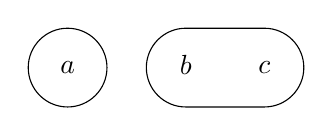
\begin{tikzpicture}[x=1mm,y=-1mm]
\draw [rounded corners=5mm] (0,0) rectangle (10,10);
\draw [rounded corners=5mm] (15,0) rectangle (35,10);
\node at (5,5) {\vphantom{Yy}$a$};
\node at (20,5) {\vphantom{Yy}$b$};
\node at (30,5) {\vphantom{Yy}$c$};
\end{tikzpicture}
\end{center}
Existential quantifiers are depicted as heavy lines that link occurrences of the same variable. The variables do not have names. For instance, if $P$ and $R$ are unary predicates and $Q$ is a binary predicate, then the formula \[∃x.¬P\,x ∧ ¬ (∃y.Q\,x\,y ∧ R\,y)\] is depicted as
\begin{center}
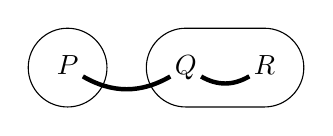
\begin{tikzpicture}[x=1mm,y=-1mm]
\draw [rounded corners=5mm] (0,0) rectangle (10,10);
\draw [rounded corners=5mm] (15,0) rectangle (35,10);
\node (p) [inner sep=0.5mm] at (5,5) {\vphantom{Yy}$P$};
\node (q) [inner sep=0.5mm] at (20,5) {\vphantom{Yy}$Q$};
\node (r) [inner sep=0.5mm] at (30,5) {\vphantom{Yy}$R$};
\path (p) edge [ultra thick, bend right] (q);
\path (q) edge [ultra thick, bend right] (r);
\end{tikzpicture}
\end{center}
Note that the heavy line for the $y$-quantifier lies entirely within the right-hand ring. If the line is pulled outside of that ring, like so 
\begin{center}
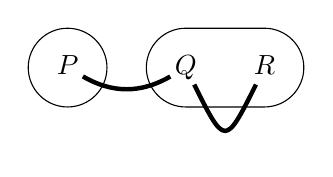
\begin{tikzpicture}[x=1mm,y=-1mm]
\draw [rounded corners=5mm] (0,0) rectangle (10,10);
\draw [rounded corners=5mm] (15,0) rectangle (35,10);
\node (p) [inner sep=0.5mm] at (5,5) {\vphantom{Yy}$P$};
\node (q) [inner sep=0.5mm] at (20,5) {\vphantom{Yy}$Q$};
\node (r) [inner sep=0.5mm] at (30,5) {\vphantom{Yy}$R$};
\path (p) edge [ultra thick, bend right] (q);
\draw [ultra thick] (q) .. controls (25,15) .. (r);
\end{tikzpicture}
\end{center}
then we are several ways to parse the existential graph, all equivalent: 
\begin{eqnarray*}
∃x.¬P\,x ∧ (∃y.¬ (Q\,x\,y ∧ R\,y))
\\
∃x.∃y.¬P\,x ∧ ¬ (Q\,x\,y ∧ R\,y) 
\\ 
∃y.∃x.¬P\,x ∧ ¬ (Q\,x\,y ∧ R\,y).
\end{eqnarray*}

\noindent Peirce's existential graphs do not have a notion of free variables; all variables are bound. 

\subsection{Branching quantifiers}

Henkin's branching quantifiers~\cite{henkin61} can be used to express certain statements that cannot be expressed within first-order logic. For instance, Hintikka~\cite{hintikka74} proposes the sentence ``some relative of each villager and some relative of each townsman hate each other'' as one that cannot be adequately captured using first-order logic, and proposes instead to write 
\[
\left(\begin{array}{ll}\forall x_1 & \exists y_1\\ \forall x_2 & \exists y_2\end{array}\right) \left((V\,x_1 ∧ T\,x_2) ⇒ (R\,x_1\,y_1 ∧ R\,x_2\,y_2 ∧ H\,y_1\,y_2)\right)
\]
The matrix of quantifiers at the beginning of this formula indicates that the witness for $y_1$ depends on $x_1$ but not on $x_2$, and that the witness for $y_2$ depends on $x_2$ but not on $x_1$. Such complex dependencies are inexpressible using the statically-scoped quantifiers of first-order logic.

It may be possible to express Hintikka's sentence using dynamically-scoped quantifiers, as suggested by the following picture.
\begin{center}
\begin{tikzpicture}[x=1mm,y=-1mm]
\ifx\verbose\undefined\else\tikzset{show grid=all}\fi
\node [inner sep=0.5mm] (x1) at (-10,-12) {$∀x_1$};
\node [inner sep=0.5mm] (y1) at (10,-8) {$∃y_1$};
\node [inner sep=0.5mm] (x2) at (0,12) {$∀x_2$};
\node [inner sep=0.5mm] (y2) at (20,8) {$∃y_2$};
\node at (0,0) {$\left((V\,x_1 ∧ T\,x_2) ⇒ (R\,x_1\,y_1 ∧ R\,x_2\,y_2 ∧ H\,y_1\,y_2)\right)$};
\draw (x1) edge [quantifieredge] (y1);
\draw (x2) edge [quantifieredge] (y2);
\draw (x1) edge [quantifieredge] (-27,-2);
\draw (x1) edge [quantifieredge] (-3,-2);
\draw (x2) edge [quantifieredge] (-16,2);
\draw (x2) edge [quantifieredge] (11,2);
\draw (y1) edge [quantifieredge] (2,-2);
\draw (y1) edge [quantifieredge] (26,-2);
\draw (y2) edge [quantifieredge] (17,2);
\draw (y2) edge [quantifieredge] (31,2);
\end{tikzpicture}
\end{center}

 

\subsection{Dynamic logic}

\newcommand{\semicolon}{\mathbin{\texttt{;}}}
\newcommand{\stsixe}{\reflectbox{\ensuremath{\exists}}} 

Groenendijk and Stokhof~\cite{groenendijk+90} describe an extension of dynamic logic~\cite{harel+00}, called dynamic predicate logic, in which quantifiers are thought of as state-modifiers. Their idea has been applied to natural language processing, to provide a compositional parsing of multi-sentence phrases. Formulas no longer denote predicates on variable interpretations, but are now \emph{relations between} variable interpretations. In other words, each formula is a program that modifies the variable interpretation as it is `executed' from left to right. For instance, `$∃x$' is an action that havocs the value of $x$. 

Vermeulen~\cite{vermeulen00} proposes an extension of dynamic predicate logic in which each variable denotes a stack of values. The action $∃x$ does not simply overwrite $x$ with an arbitrary value, but rather pushes an arbitrary value onto $x$'s stack. The new action $x\stsixe$ pops from $x$'s stack. Writing `$φ_0\semicolon φ_1$' to denote relational composition, his system can express our formula~\eqref{eq:sentence1} in a form in which the quantifiers are pushed `inside' in a normalised way, like so: 
\[
∃x \semicolon (0 < x) \semicolon ∃y \semicolon (x < y) \semicolon x\stsixe \semicolon (y < z) \semicolon y\stsixe \semicolon (z < 4)
\]

\noindent Vermeulen's system is able to express formulas using fewer variable names. It is very different from our proposed system, which does not involve a dynamic semantics.

\subsection{Milner's bigraphs}

Our dynamically-scoped quantifiers are somewhat reminiscent of Milner's bigraphs~\cite{milner09}. Here is formula~\eqref{eq:sentence3} again, drawn this time as a bigraph.

\begin{center}
\begin{tikzpicture}[x=1mm,y=-1mm]
\ifx\verbose\undefined\else\tikzset{show grid=all}\fi


\draw[thick] (-8,0) ellipse (5 and 3);
\node at (-8,0) {$0<x$};
\draw[thick] (4,0) ellipse (5 and 3);
\node at (4,0) {$x<y$};
\node at (-2,-4) {$∧$};

\draw[thick] (-2,0) ellipse (13 and 6);

\draw[thick] (18,0) ellipse (5 and 3);
\node at (18,0) {$y<z$};
\node at (12,-5) {$∧$};

\draw[thick] (4,0) ellipse (21 and 8);

\draw[thick] (32,0) ellipse (5 and 3);
\node at (32,0) {$z<4$};
\node at (26,-6) {$∧$};

\draw[thick] (10,0) ellipse (29 and 10);

\node [inner sep=0.4mm, fill=black, circle] (p1) at ($(-8,0)+(30:5 and 3)$) {};
\node [inner sep=0.4mm, fill=black, circle] (p2) at ($(4,0)+(150:5 and 3)$) {};
\path (p1) edge [draw=Green, bend right, auto=right] node {$x$} (p2);


\node [inner sep=0.4mm, fill=black, circle] (p3) at ($(4,0)+(40:5 and 3)$) {};
\node [inner sep=0.4mm, fill=black, circle] (p4) at ($(18,0)+(140:5 and 3)$) {};
\path (p3) edge [draw=Green, bend right, auto=right] node {$y$} (p4);


\node [inner sep=0.4mm, fill=black, circle] (p5) at ($(18,0)+(70:5 and 3)$) {};
\node [inner sep=0.4mm, fill=black, circle] (p6) at ($(32,0)+(140:5 and 3)$) {};
\node (z1) at (32,9) {$z$};
\path (p5) edge [draw=Green, bend right, pos=0.4] node [inner sep=0mm] (z2) {} (z1);
\path (p6) edge [draw=Green, bend right] (z2);

\end{tikzpicture}
\end{center}

\noindent Note that each \emph{atomic control} has one \emph{port} per free variable. The \emph{link} corresponding to the $z$ variable is an \emph{outer name}, so that it can later be bound when this bigraph is substituted into a broader context.

\subsubsection*{Acknowledgements} The author thanks Thomas Göthel for many helpful suggestions and stimulating discussions, and acknowledges the support of a postdoctoral scholarship from the German Academic Exchange Service (DAAD).

\bibliographystyle{abbrv}
\bibliography{/Users/jpw48/Dropbox/john.bib}

\end{document}